\documentclass{beamer}
\usepackage{fontspec}
\usepackage{fontspec}
\usepackage{xunicode}
\usepackage{caption}
\usepackage{xltxtra}
\usepackage{xecyr}
\usepackage{hyperref}
\setmainfont[Mapping=tex-text]{DejaVu Serif}
\setsansfont[Mapping=tex-text]{DejaVu Sans}
\setmonofont[Mapping=tex-text]{DejaVu Sans Mono}
\usepackage{polyglossia}
\setdefaultlanguage{russian}
\usepackage{graphicx}
\usepackage{listings}

\mode<presentation> {
\usetheme{Singapore}
\usecolortheme{dove}

\setbeamertemplate{footline}[page number]
%\setbeamertemplate{caption}[numbered]
\setbeamertemplate{caption}{\insertcaption}
}


\usepackage{graphicx}
\usepackage{booktabs}

\title{Построение генетических карт по неполным и
зашумленным данным}
\author{Алина Крамар\\
  { \footnotesize \textcolor{gray}{группа 545\\ руководитель Сысоев
      С.С\\ рецензент Добрынин П.B.}}}
\institute{Санкт-Петербургский государственный университет}
\date{\today}

\begin{document}
\newcommand{\genmap}{\textbf{genmap}}

\begin{frame}
\titlepage
\end{frame}

\begin{frame}
  \frametitle{Необходимые определения}

  \begin{columns}
    \column{.5\textwidth}
    \begin{itemize}
    \item геном
    \item аллель маркер
    \item кроссинговер
    \item \underline{генетическая карта}
    \end{itemize}

    \column{.5\textwidth}
    \begin{figure}
      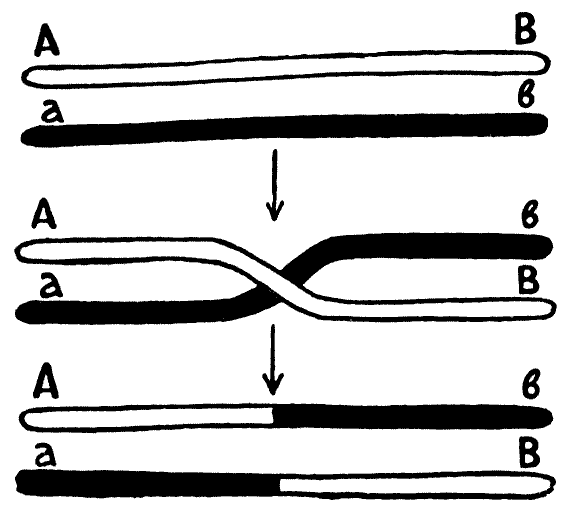
\includegraphics[width=0.4\textwidth]{cross.png}
      \caption{Кроссинговер}
    \end{figure}
    \begin{figure}
      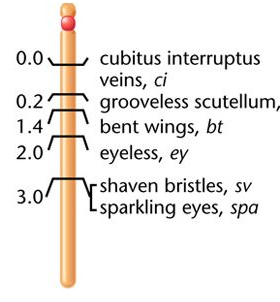
\includegraphics[width=0.4\textwidth]{map.png}
      \caption{Генетическая карта}
    \end{figure}

  \end{columns}
\end{frame}

\begin{frame}
  \frametitle{Существующие решения}
  \begin{itemize}
  \item CRIMAP

    Экспоненциальная сложность от количества особей в родословной.
  \item FASTLINK

    Экспоненциальная сложность от количества маркеров.
  \item \genmap

    Полиномиальная сложность от количества особей и маркеров.
  \end{itemize}
\end{frame}

\begin{frame}
  \frametitle{Постановка задачи}
  Разработать новый алгоритм генетического картирования на базе метода
  прямого извлечения данных \genmap.

  \medskip

  Задачи:
  \begin{itemize}
  \item Доработка алгоритма прямого извлечения данных \genmap.
  \item Верификация полученного алгоритма.
    \begin{itemize}
    \item Моделирование и генерация тестовых данных.
    \item Сравнение c существующими алгоритмам.
    \end{itemize}
  \end{itemize}
\end{frame}

\begin{frame}
  \frametitle{Улучшение \genmap}

  Недостатки:
  \begin{itemize}
  \item Неустойчивость к вариациям входных данных.
  \item Неоптимальная реализация.
  \item Неправильный результат в случае кратного кроссинговера.
  \end{itemize}

  Что улучшили:
  \begin{itemize}
  \item Работа с ``плохими'' данными.
  \item Уточнение карты.
  \item Учёт кратных кроссинговеров.
  \end{itemize}
\end{frame}

\begin{frame}
  \frametitle{Генерация тестовых данных}
  Ситетические vs. реальные данные.

  Много параметров:
  \begin{itemize}
  \item Стратегия кроссинговера.
  \item Численные параметры родословной.
  \item Ошибки секвенирования.
  \end{itemize}
\end{frame}

\begin{frame}
  \frametitle{Результаты сравнения алгоритмов}
 % +----------------+---------------+---------------+---------------+
 % |                |Genmap2        |FASTLINK       |CRIMAP         |
 % |Особи/Маркеры   |               |               |               |
 % +----------------+---------------+---------------+---------------+
 % |200/30          |0.3 секунд     |10 минут       |1 час          |
 % |                |               |               |               |
 % +----------------+---------------+---------------+---------------+
 % |200/50          |0.3 секунды    |10 минут       |\infty         |
 % |                |               |               |               |
 % +----------------+---------------+---------------+---------------+
 % |400/40          |6 секунд       |\infty         |3 дня          |
 % |                |               |               |               |
 % +----------------+---------------+---------------+---------------+
  % This LaTeX table template is generated by emacs 24.3.1

  \begin{tabular}{|l|l|l|l|}
    \hline
    & Genmap2 & FASTLINK & CRIMAP \\
    Особи/Маркеры & & & \\
    \hline
    200/30 & 0.3 секунд & 10 минут & 1 час \\
    & & & \\
    \hline
    200/50 & 0.3 секунды & 10 минут & $ \infty $ \\
    & & & \\
    \hline
    400/40 & 6 секунд & $ \infty $ & 3 дня \\
    & & & \\
    \hline
  \end{tabular}
\end{frame}

\begin{frame}
  \frametitle{Результаты}
  Реализован более хороший алгоритм на основе \genmap. Проведена его
  верификация.
  \begin{itemize}
  \item Использованы естественные и синтетические данные.
  \item Экспериментально показаны его сильные стороны.
  \item Произведено сравнение с аналогами.
  \end{itemize}

  \bigskip

  Результаты работы были представлены на конференции
  \textbf{СПИСОК-2014}.
\end{frame}

\end{document}

%%% Local Variables:
%%% coding: utf-8
%%% mode: latex
%%% TeX-engine: xetex
%%% End:
